\documentclass[12pt, a4paper]{article}
\usepackage{scrextend}
\usepackage[utf8]{inputenc}
\usepackage[polish]{babel}
\usepackage[T1]{fontenc}%polskie znaki
\usepackage[utf8]{inputenc}%polskie znaki
\usepackage{geometry}
\usepackage{float}
\usepackage{enumitem}
\usepackage{hyperref}
\usepackage{graphicx}
\usepackage{amsmath}
\usepackage{tabularx}
\usepackage{pdflscape}


\renewcommand{\baselinestretch}{1.5}


\begin{document}

\begin{flushleft}
    Damian Koper \textbf{241292} \\
\end{flushleft}
\vspace{1cm}
{
    \centering
    {\Huge\scshape\bfseries Modelowanie i analiza systemów informatycznych }\\
    \large{Logika Temporalna i Automaty Czasowe - konstrukcja i weryfikacja czasowych automatów UPPAAL 2.}\\
    \vspace{0.5cm}
}
\newcounter{ex}
\setcounter{ex}{0}

\newcounter{fm}
\setcounter{fm}{0}

\newcommand{\ex}[1]{
    \refstepcounter{ex}{
        \noindent\normalfont\Large\bfseries Zadanie \arabic{ex}.
    } \\
    #1
}

\newcommand{\fm}[4]{
    \refstepcounter{fm}{
        \noindent\normalfont\large\bfseries Formuła \arabic{fm} \normalsize\normalfont
\begin{itemize}
    \item[UPPALL:] \texttt{#1}
    \item[CTL:] #2
    \item[Opis:] #3
    \item[Wynik:] #4
\end{itemize}
    }
    \vspace{1cm}
}

\ex{Serwer, klienty i sesje}
\begin{figure}[H]
    \centering
    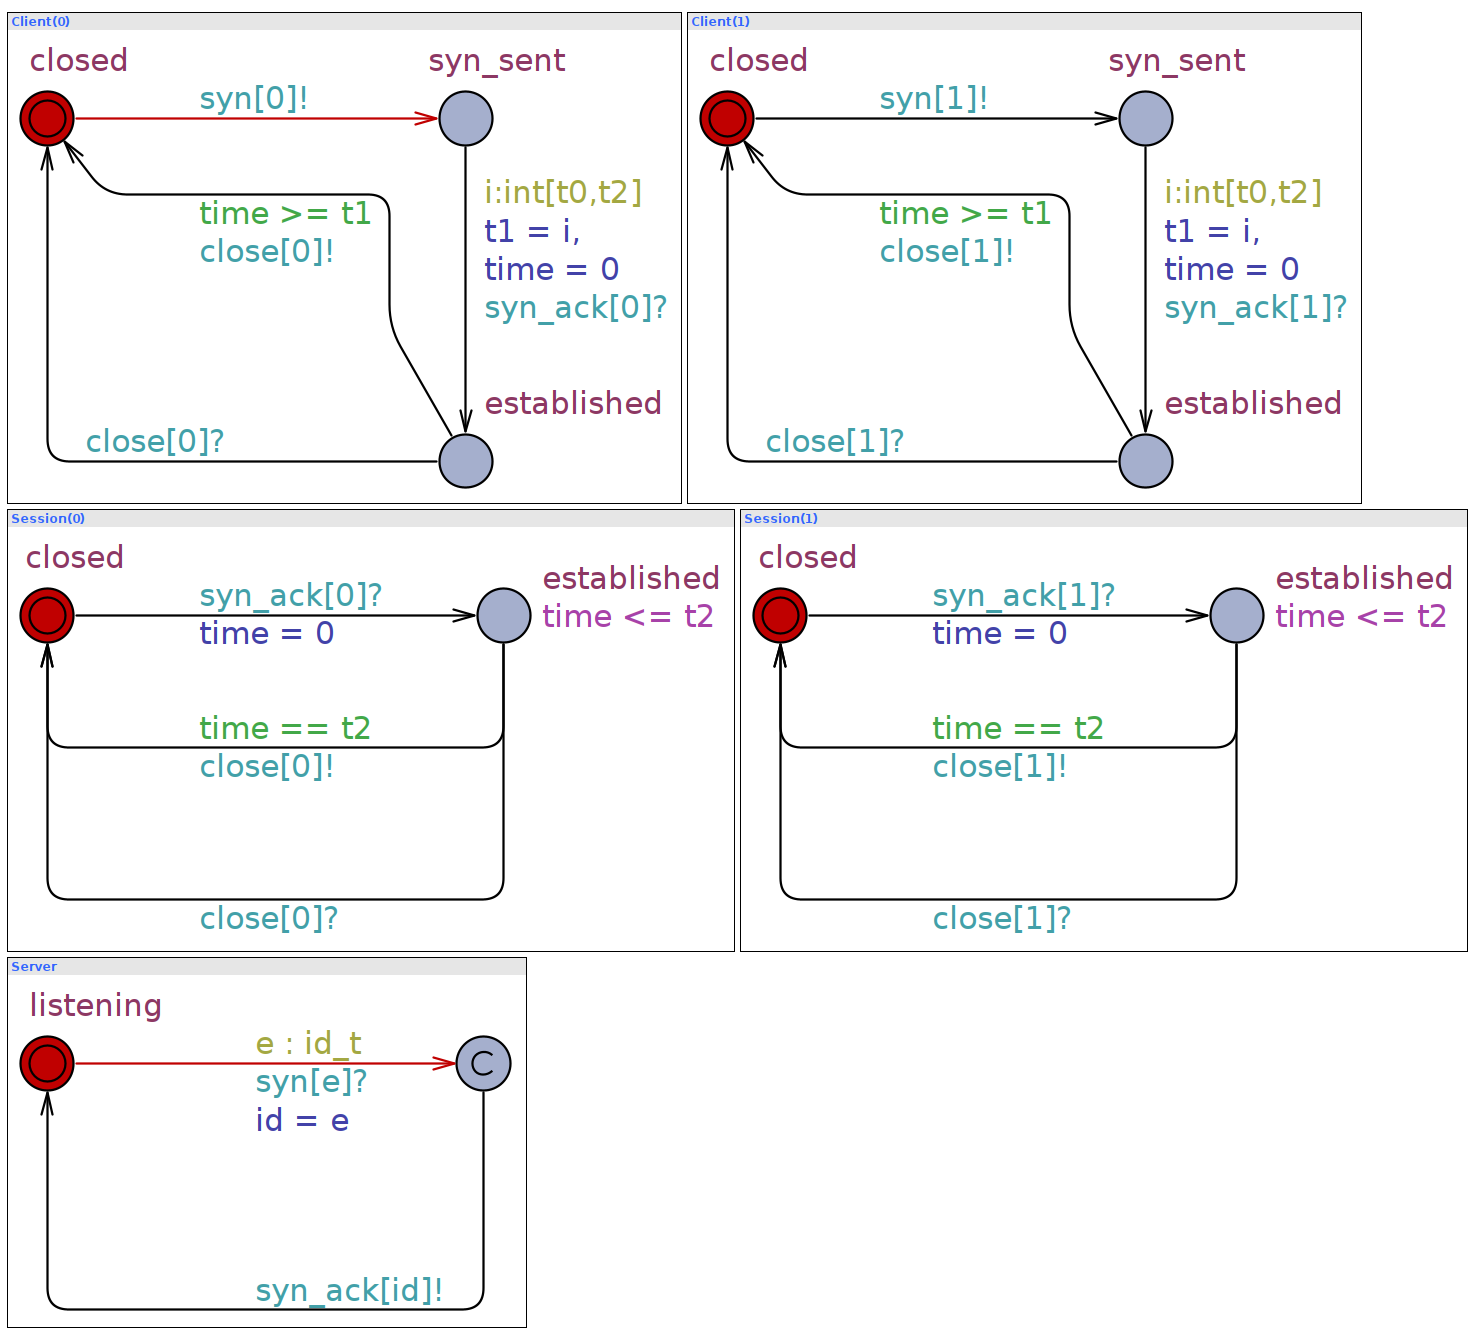
\includegraphics[width=0.9\linewidth]{../../lab13/ex_1_2}
\end{figure}
\clearpage
\ex{Weryfikacja automatów z zadania 1}

\fm
{A[] forall(x:id\_t) Client(x).established imply Client(x).time <= t2}
{$AG(\prod\limits_{x=0}^n (Client(x).established \implies Client(x).time \le t_2))$}
{Na pewno zawsze dla wszystkich klientów kiedy Client(x).established, Client(x).time $\le t_2$.}
{True}

\fm
{E<> forall(x:id\_t) Client(x).established and Client(x).time == t2}
{$EF(\prod\limits_{x=0}^n (Client(x).established \wedge Client(x).time = t_2))$}
{Jest możliwe, że kiedyś dla wszystkich klientów Client(x).established i Client(x).time = t2.}
{True}

\clearpage

\fm
{A<> forall(x:id\_t) (Client(x).established imply Client(x).time >= t0)}
{$AF(\prod\limits_{x=0}^n (Client(x).established \wedge Client(x).time = t_0))$}
{Zawsze kiedyś dla wszystkich klientów w Client(x).established - Client(x).time $\ge t_0$.}
{True}

\fm
{E<> exists(x:id\_t) Session(x).established and Session(x).time > t2}
{$EF(\bigcup\limits_{x=0}^n (Session(x).established \wedge Session(x).time > t_2))$}
{Jest możliwe, że kiedyś istnieje sesja, gdzie Session(x).established i Session(x).time $> t_2$.}
{False - nie może istnieć sesja dłuższa od $t_2$.}

\clearpage

\fm
{A[] sum(x:id\_t) Client(x).syn\_sent <= 1}
{$AG((\sum\limits_{x=0}^n Client(x).syn\_sent) \le 1)$}
{Zawsze w przyszłości naraz zapytanie o połączenie może wysłać tylko jeden klient.}
{True}

\fm
{E<> (sum(x:id\_t) Client(x).established) == n}
{$EF((\sum\limits_{x=0}^n Client(x).established) = n)$}
{Jest możliwe, że kiedyś wszystkie klienty będą na raz połączone.}
{True}
\clearpage

\fm
{E<> forall(x:id\_t) Client(x).established}
{$EF(\prod\limits_{x=0}^n (Client(x).established)$}
{Jest możliwe, że kiedyś wszystkie klienty będą na raz połączone. Inny zapis.}
{True}

\fm
{Session(0).established --> Session(0).closed}
{$AG(Session(0).established \implies AF(Session(0).closed))$}
{Sesja 0 na pewno będzie kiedyś zamknięta.}
{True}
\clearpage

\fm
{A[] forall(x:id\_t) (Client(x).established imply Session(x).established)}
{$AG(\prod\limits_{x=0}^n (Client(x).established \implies Session(x).established))$}
{Zawsze w przyszłości dla każdego klienta w Client(x).established - Session(x).established. Stan klienta i sesji jest zawsze zsynchronizowany.}
{True}

\end{document}
